\chapter{Практические исследования} 
\label{chapter3}

В данной главе рассмотрены экспериментальные результаты, полученные в течение работы. 

Наша основная задача, как было описано в главе посвященной теоретическим исследованиям, заключается в том, чтобы быстро выбирать наилучший алгоритм, основываясь на входных данных.   
Для этого необходимо сначала собрать довольно много данных по времени их работы на разных входных данных. 

\section{Виды входных данных}
Рассмотрим какие именно входные данные будем рассматривать. 
\begin{itemize}
	\item Случайный точки в гиперкубе.
	\item Точки на одном ранге.
	\item Точки часто имеею одинаковый критерии. 
	\item Каждая точка имеет отличный от других ранг.
	\item Крайние случаи с шумами.
\end{itemize}

\section{Детали гибридизации}
Примитивный избиратель алгоритмов, который принимает решение в самом начале, основываясь на всех данных в целом.

Следующая идея сбора информации: сделаем дампы в момент каждого рекурсивного вызовов алгоритма Fast и сравним время сортировки этих подмножеств алгоритмами.

\section{Формат экспериментов}
Будем засекать время на каждом интересующем нас множестве данных. Если время незначительно, запускаем алгоритм на одних и тех же данных $2^i$ раз, где i - количество пренебрежимо маленьких замеров времени. 

Обозначим $T_\text{Fast}$ - как время за которое алгоритм Fast отсортировал экспериментальное множество точек S, $T_\text{BOS}$ - время за которое справился алгоритм BOS.  
$T_\text{max} = max (T_\text{BOS}, T_\text{Fast})$

Оценивать будем с помощью графика, где по абсцисе будет мощность множества S для которого проводился эксперимент. По ординате будет $\frac{T_\text{BOS} - T_\text{Fast}}{T_\text{max}}$.

\section{Результаты экспериментов}

На данном этапе работы были исследованы случайные точки в гиперкуб и точки на одном ранге. 

\subsection{Случайные точки в гиперкубе}


Эксперименты были запущены для N = 100000 и M = {4, 6, 8, 10, 12, 14, 16, 18, 20}

\subsubsection{Замеры}
\begin{center}
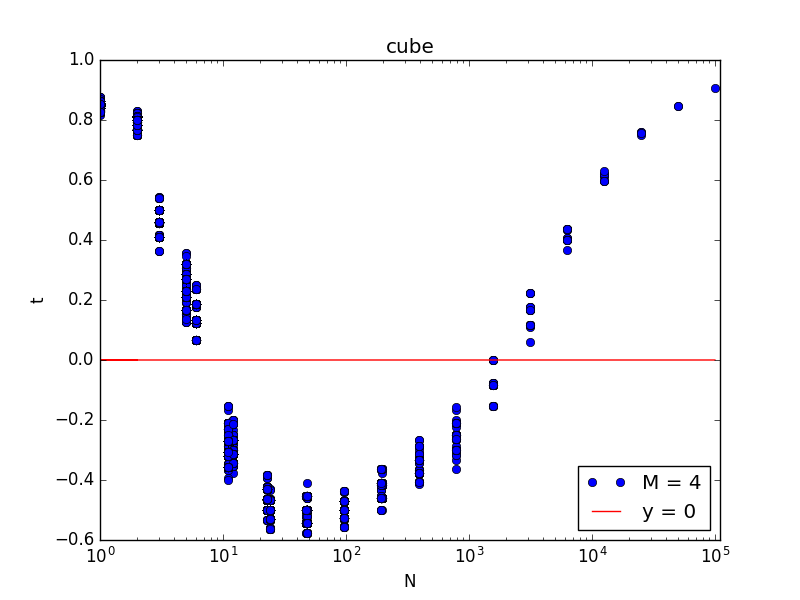
\includegraphics[width = 8cm]{pic/cube_m=4}
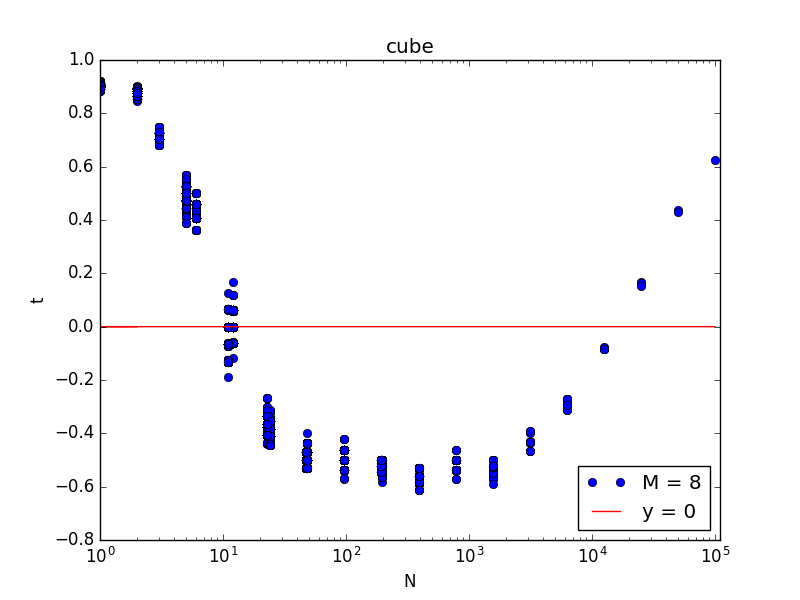
\includegraphics[width = 8cm]{pic/cube_m=8}
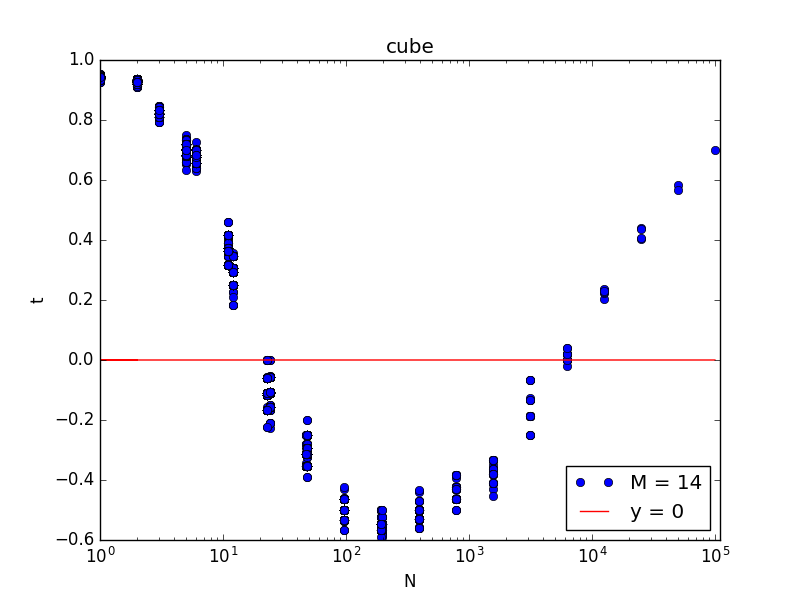
\includegraphics[width = 8cm]{pic/cube_m=14}
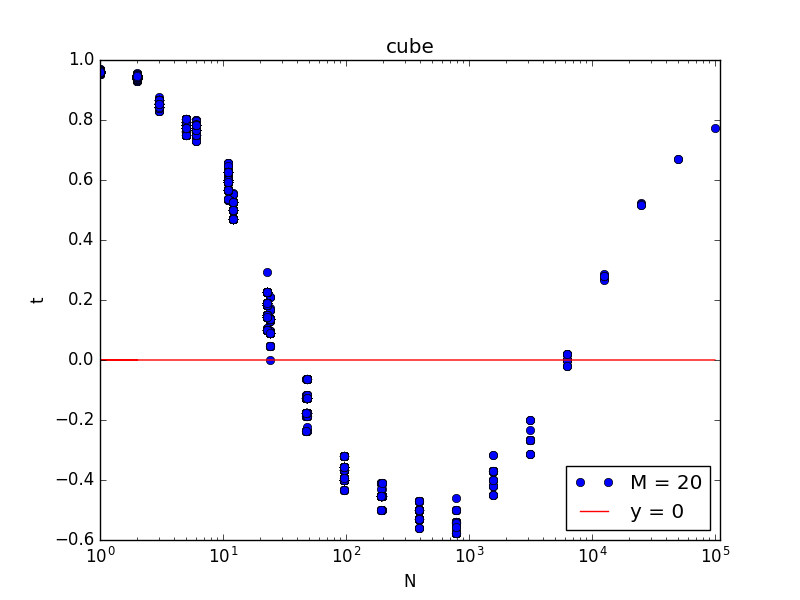
\includegraphics[width = 8cm]{pic/cube_m=20}
\end{center}

\subsubsection{Левая и правая границы}
\begin{center}
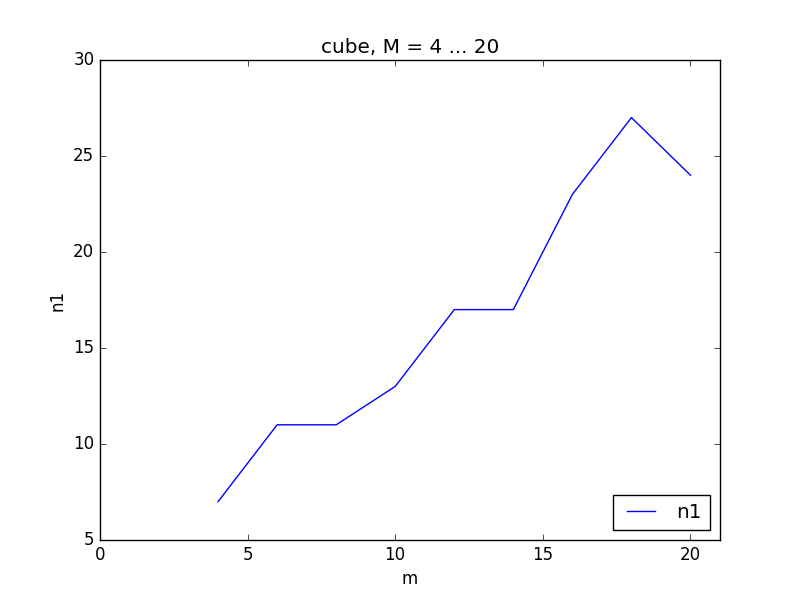
\includegraphics[width = 8cm]{pic/cube_n1-}
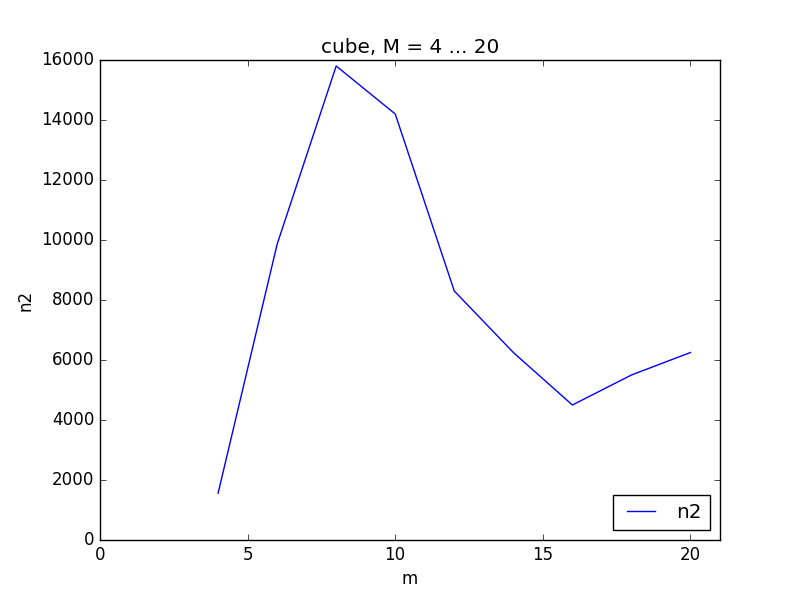
\includegraphics[width = 8cm]{pic/cube_n2-}
\end{center}

\subsubsection{Выводы}
Левая граница похожа на линейную с коэффициентом 4/3

Правая граница ведет себя непонятным образом с максимумом около 8. 


\subsection{Точки одного ранга}
Эксперименты были запущены для N = 100000 и M = {4, 8, 10, 14, 16, 18, 20}

\subsubsection{Замеры}
\begin{center}
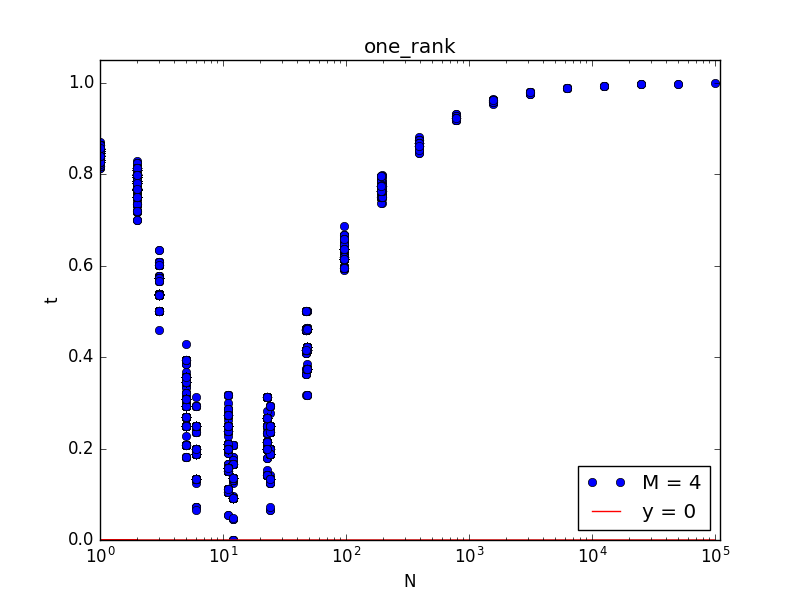
\includegraphics[width = 8cm]{pic/one_rank_m=4}
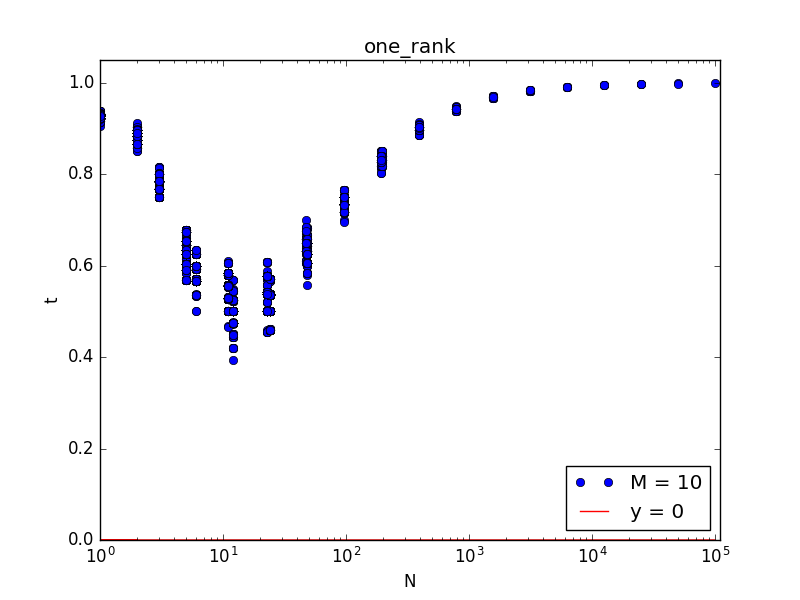
\includegraphics[width = 8cm]{pic/one_rank_m=10}
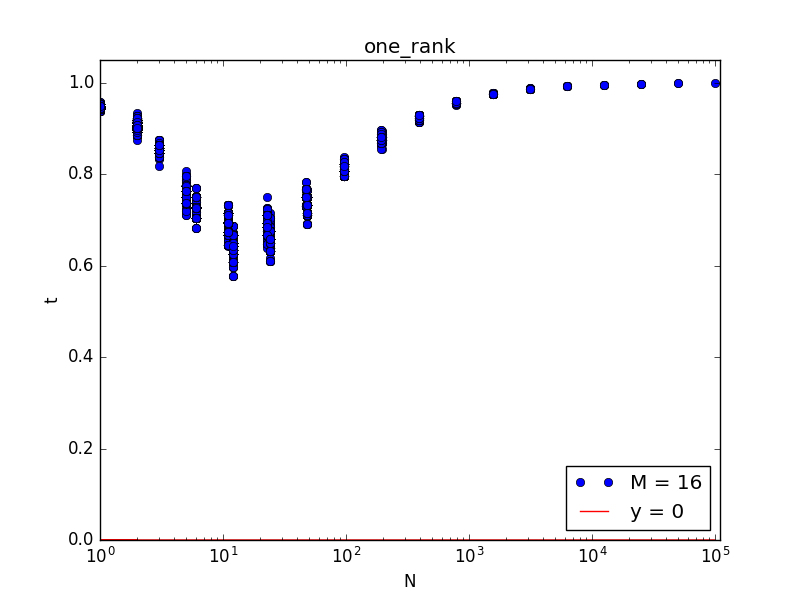
\includegraphics[width = 8cm]{pic/one_rank_m=16}
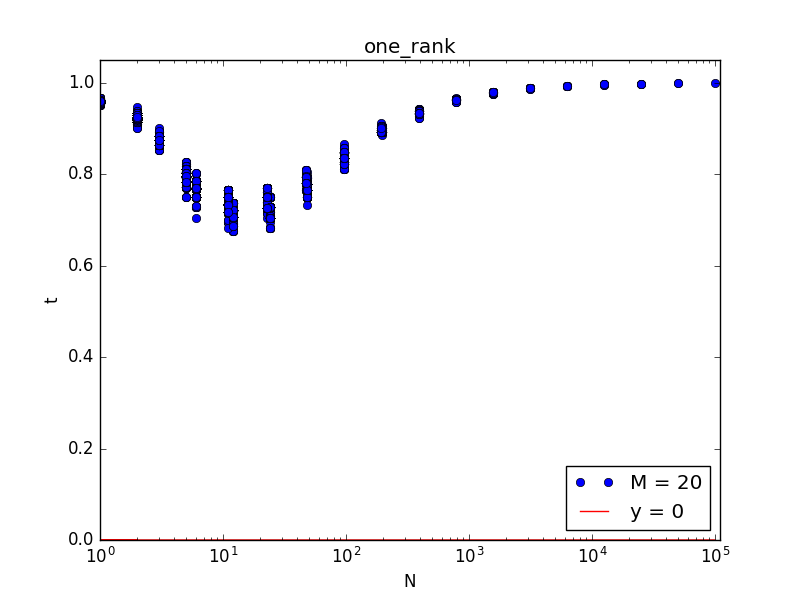
\includegraphics[width = 8cm]{pic/one_rank_m=20}
\end{center}

\subsubsection{Выводы}
BOS работает всегда хуже.


\section{Дальнейшие действия}
Запустить на других N и M, чтобы проверить гипотезы. 

Исследовать поведение в крайних случаях с шумами. Например, взять однофронтовый набор точке и добавить шумы, при этом сколько конкретно шума - параметр, который надо будет подвигать. 


\section{Выводы}
\begin{itemize}
	\item Соотношение времени - функция выпуклая вниз. 
	\item Чем больше разбросаны точки, тем лучше работает BOS
	\item Чем меньше фронтов, тем быстрее работают оба алгоритма
	\subitem у BOS это в рамках константы
	\subitem У Fast логарифмическое ускорение
\end{itemize}

Важная идея заключается в том, что с уменьшением числа фронтов функция соотношений времени работы поднимается и смещается влево. И если научится предсказывать примерное число фронтов, то можно понять, в какой момент переключать алгоритм. 